\subsection{Evaporation N}
	Until now the black hole could radiate an infinit amount of energy. This is of course not physically correct. We will now resore the dynamical gravity so that the mass becomes time independent. This means, it is no longer reasonable to set the Schwarzschild radius to one. From now on $r_s= 2GM$.	
	
	So the old definition of the black hole's energy was that is generated translations of $t$ in the Schwarzschild geometry. But in the general relativity it doesn't work any more to attach this definition to the coordinates.
	
	In an asymtotical flat space and using Hamilton formalism while the general relativity is inlcuded, the energy is an integration over the boundary at the two sphere at $r\rightarrow \infty$. In the Penrose diagram, this would be the $i^0$ boundary. It is also called the ADM energy\footnote{cherished to Arnowitt, Deser and Misner} and is not only conserved but for a black hole with mass $M$, the ADM energy is also $M$, if it was formed form a collapsing shell. 
	
	\begin{figure} [t]
		\begin{center}
			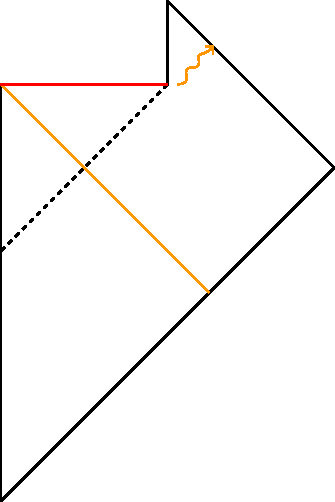
\includegraphics[scale=0.7]{evappen}
			\caption{This is the Penrose diagram for a black hole with Hawking radiation formed by a collapsing shell of photons (yellow line). The red line is the singularity and the radiation is the curvy yellow line going towards positiv null infinty.} \label{penrose_hawking}
		\end{center}
	\end{figure}
		
	Now we might be able to calculate how long a black hole lives.
	First we need the total energy disposal:
	\begin{align}
		\frac{\diff E}{\diff t} =
		\sum_{\ell, m} \int_{0}^{\infty} \frac{\diff \omega}{2 \pi}
		\frac{\omega P_{abs}(\omega,\ell)}{e^{\beta \omega} - 1}
	\end{align}
	But for computing $P_{abs}$ we would have to solve the differential equation from \eqref{schroedinger_eq} which is analytically impossible. It can be solved numerically though, but for us an approximation is sufficient. It starts with $\omega \leq \frac{1}{r_s}$. Since $P_{abs}$ grows exponentially in $\ell$ and $\omega r_s \leq 1$ we can make a taylor expansion and get
	\begin{align}
		P_ {abs}(\omega, \ell=0) = (\omega r_s)^2
	\end{align} 
	while all $\ell > 0$ can be neglected.
	This means, we now just have get the prefactor of the integral
	\begin{align}
		\frac{\diff E}{\diff t} \sim \int_{0}^{\infty} \frac{\diff \omega}{2\pi} \frac{\omega^3 r_s^2}{e^{\beta \omega}-1}
	\end{align}
	by substituting $\beta \omega$ with $x$, and then plugging in the definition of $\beta$ so we get:
	\begin{align}
		\frac{\diff E}{\diff t} \sim \frac{r_s^2}{2 \pi \beta^4} \int_{0}^{\infty} \diff x \frac{x^3}{e^{x}-1}
		= \frac{r_s^2}{2 \pi (4 \pi r_s)^4} \int_{0}^{\infty} \diff x \frac{x^3}{e^{x}-1}
	\end{align}
	which then is resulting in the following relationsship:
	\begin{align}
		\frac{\diff E}{\diff t} \approx \frac{C_1}{r_s^2}
	\end{align}	
	with the constant $C_1$. Using the fact, that the mass decreases by energyloss, a function of the mass dependent on time must obey
	\begin{align}
		\frac{\diff M}{\diff t} = -\frac{C_2}{(GM)^2} 
	\end{align}		
	which can be integrated from the initial mass to zero and from zero time to moment, when the black hole has completely evaporated. By the way, $C_2$ is just another constant containing $C_1$. This will lead to the relation:
	\begin{align}
		t_{\text{evap}} \sim G^2 M^3
	\end{align}
	If you plug in the mass of the sun ($M_s \approx 10^{30} \unit{kg}$) one will get approximatly $5 \cdot 10^{58}$ years a black hole with this mass would live until it evaporates. By comparing this to the assumed age of our universe $13.8 \cdot 10^{9}$ years, we get an idea of how tiny a black hole would have be, for to check the evaporation experimentally. Clearly astronomical black holes are way to heavy to observe it.
	
	The Penrose diagram inkluding this radiation can be seen in \textbf{Figure \ref{penrose_hawking}}.
	\FloatBarrier
	%hawkings paper [2]

	%\clearpage